\documentclass[12pt]{article}

%AMS-TeX packages
\usepackage{amssymb,amsmath,amsthm, color} 
%geometry (sets margin) and other useful packages
\usepackage[margin=0.75in]{geometry}
\usepackage{graphicx}
\usepackage{bm}
%\usepackage{graphicx,ctable,booktabs}
%\usepackage{mathrsfs, bbm}  
\usepackage{hyperref}
% \usepackage{algorithmic}
% \usepackage{algorithm2e}
% \usepackage{algorithms}

\newcommand\independent{\protect\mathpalette{\protect\independenT}{\perp}}
\def\independenT#1#2{\mathrel{\rlap{$#1#2$}\mkern2mu{#1#2}}}


\usepackage{listings}

\newcommand{\br}{{\mathbb R}} 
\newcommand{\bc}{{\mathbb C}} 
\newcommand{\bd}{{\mathbb D}} 
\newcommand{\bq}{{\mathbb Q}} 
\newcommand{\bn}{{\mathbb N}} 
\newcommand{\bz}{{\mathbb Z}} 
\newcommand{\supp}{{\text{supp} \ }} 

\newtheorem{proposition}{Proposition}[section]
\newtheorem{definition}[proposition]{Definition}
\newtheorem{conjecture}[proposition]{Conjecture}
\newtheorem{lemma}[proposition]{Lemma}
\newtheorem{corollary}[proposition]{Corollary}
\newtheorem{theorem}[proposition]{Theorem}
\newtheorem{remark}[proposition]{Remark} 

\newcommand{\eps}{{\epsilon}} 
\newcommand{\vp}{{\varphi}} 
\newcommand{\ip}[2]{\left \langle #1, #2 \right\rangle}
\newcommand{\norm}[1]{\left \lVert #1 \right \rVert}
\newcommand{\Var}{\text{Var}} 


%
%Fancy-header package to modify header/page numbering 
%
\usepackage{fancyhdr}
\pagestyle{fancy}
%\addtolength{\headwidth}{\marginparsep} %these change header-rule width
%\addtolength{\headwidth}{\marginparwidth}
\renewcommand{\headrulewidth}{.3pt} 
\renewcommand{\footrulewidth}{.3pt}
%\setlength\voffset{-0.25in}
\setlength\textheight{648pt}

\begin{document}

\title{Fast and accurate p-values for SCEPTRE: Preliminary Ideas}
\author{Gene}
\date{January 3, 2023}

\maketitle
\thispagestyle{empty}

For convenience, all resampling distributions are stored in the folder \verb|figures/|. There is one figure per dataset and effective sample sizes, each containing ten panels corresponding to ten pairs. Browsing these is illuminating, and I will summarize some of the main findings next. 

\section[Exploration]{Exploration of resampling distributions}

\subsection{Bumpy-ness of the resampling distributions}

\paragraph{Many of the resampling distributions are bumpy, but a given resampling distribution need not be bumpy throughout.} For a given resampling distribution, define the \textit{bumpy region} $\mathcal B \subseteq [0,1]$ of quantiles $q \in \mathcal B$ where the distribution is bumpy. For example, Figure~\ref{fig:schraivogel-7}  shows the resampling distributions for the Schraivogel pairs with effective sample size 7. I would estimate that the bumpy regions of these ten distributions are roughly $[0,1], [0,1], [0,1], \varnothing, \varnothing, [0, 0.6], \varnothing, [0, 0.6], \varnothing$, and $\varnothing$, respectively.

\paragraph{Bumpy-ness tends to decrease with effective sample size, but the correlation is imperfect. In particular, it is possible to have non-bumpy distributions for low effective sample sizes and bumpty distributions for higher effective sample sizes.} In Figure~\ref{fig:schraivogel-7}, corresponding to an effective sample size of 7, half of the distributions have $\mathcal B = \varnothing$, i.e. are not bumpy at all. Another two of the distributions have non-bumpy right tails. On the other hand, there is a somewhat bumpy Papalexi pair with effective sample size equal to 30. This suggests that we cannot rely so much on the effective sample size to predict whether a resampling distribution will be bumpy. In particular, we might even be able to push the QC threshold for effective sample size lower, and then produce $p$-values for the non-bumpy distributions. This is worth it only if we can gain power, so perhaps we shouldn't pursue this in the short run.

\paragraph{The bumps follows a somewhat regular pattern.}

The bumps appear to be about equally spaced, and their peaks appear to form something like a skew-t distribution. 

\subsection{The shapes of the non-bumpy distributions}

\paragraph{Many non-bumpy distributions look roughly normal; others look roughly skew-t; others look like neither.} Most of the distributions have mean roughly zero and standard deviation roughly one, but there are exceptions. The first and second Schraivogel distribution with effective sample size 25 (Figure~\ref{fig:schraivogel-25}) have standard deviations of roughly a half. The sixth Papalexi distribution with effective sample size of 30 (Figure~\ref{fig:papalexi-30}) is centered roughly on -3. The skew-$t$ is probably appropriate in many cases when $N(0,1)$ is not. The skew is typically to the right (i.e. longer right tails).Even the skew-$t$ fit may not always be appropriate. For example, the last Schraivogel distribution with effective sample size 25 (Figure~\ref{fig:schraivogel-25}) appears to have an abnormally long right tail even for a skew-t distribution. Other Schraivogel distributions (not shown) exhibit a similar phenomenon.

\begin{figure}[h!]
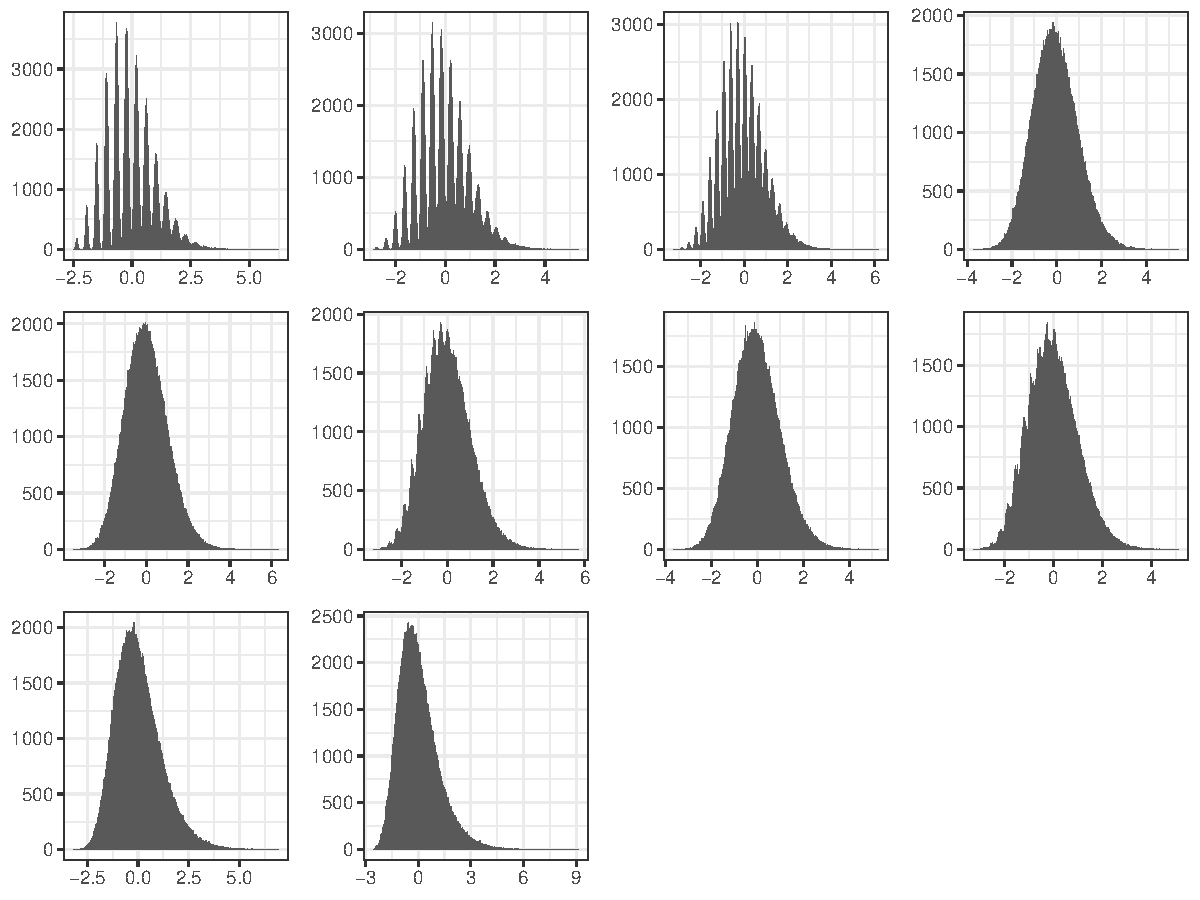
\includegraphics[width = \textwidth]{figures/schraivogel_enhancer_screen_chr11_gene_eff_ss_7.pdf}
\caption{Schraivogel data (effective sample size = 7).}
\label{fig:schraivogel-7}
\end{figure}

\begin{figure}
	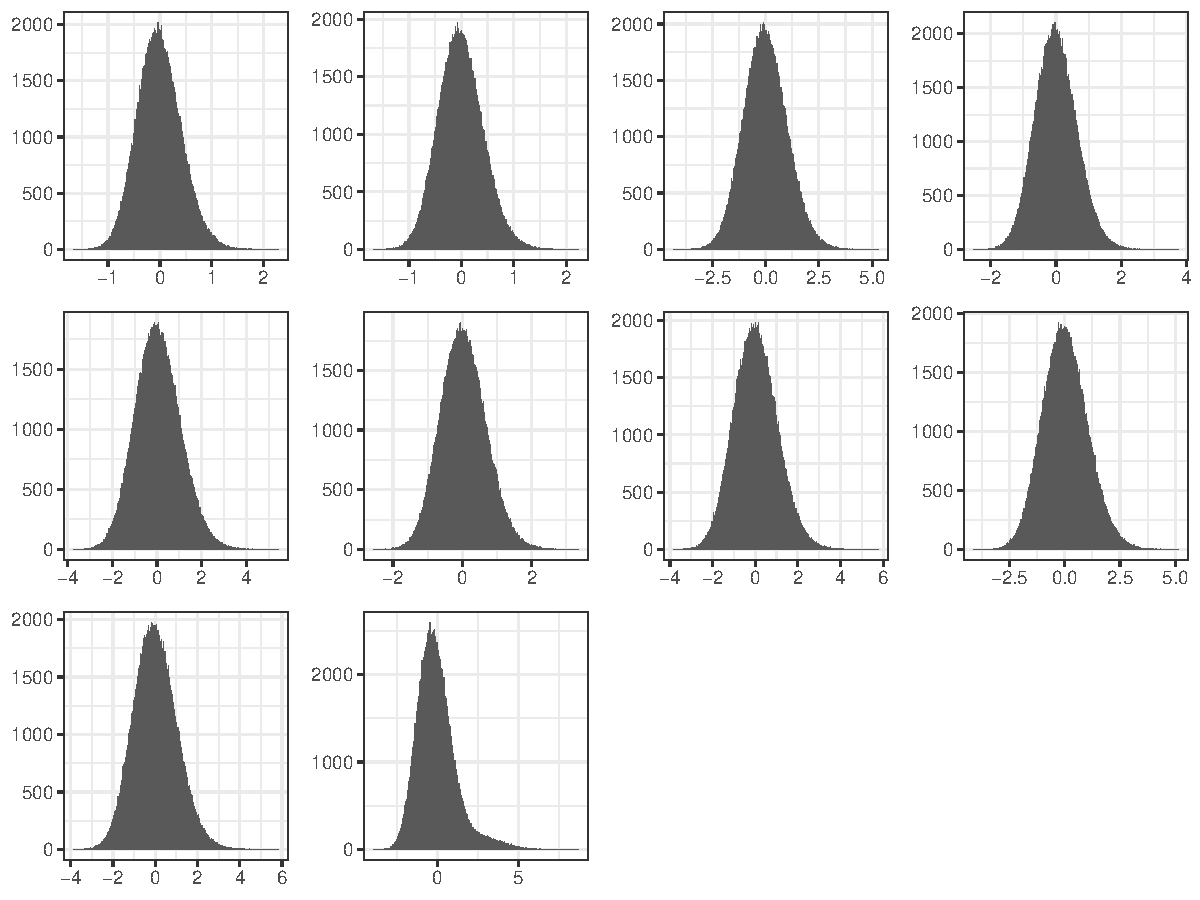
\includegraphics[width = \textwidth]{figures/schraivogel_enhancer_screen_chr11_gene_eff_ss_25.pdf}
	\caption{Schraivogel data (effective sample size = 25).}
	\label{fig:schraivogel-25}
\end{figure}

\begin{figure}
	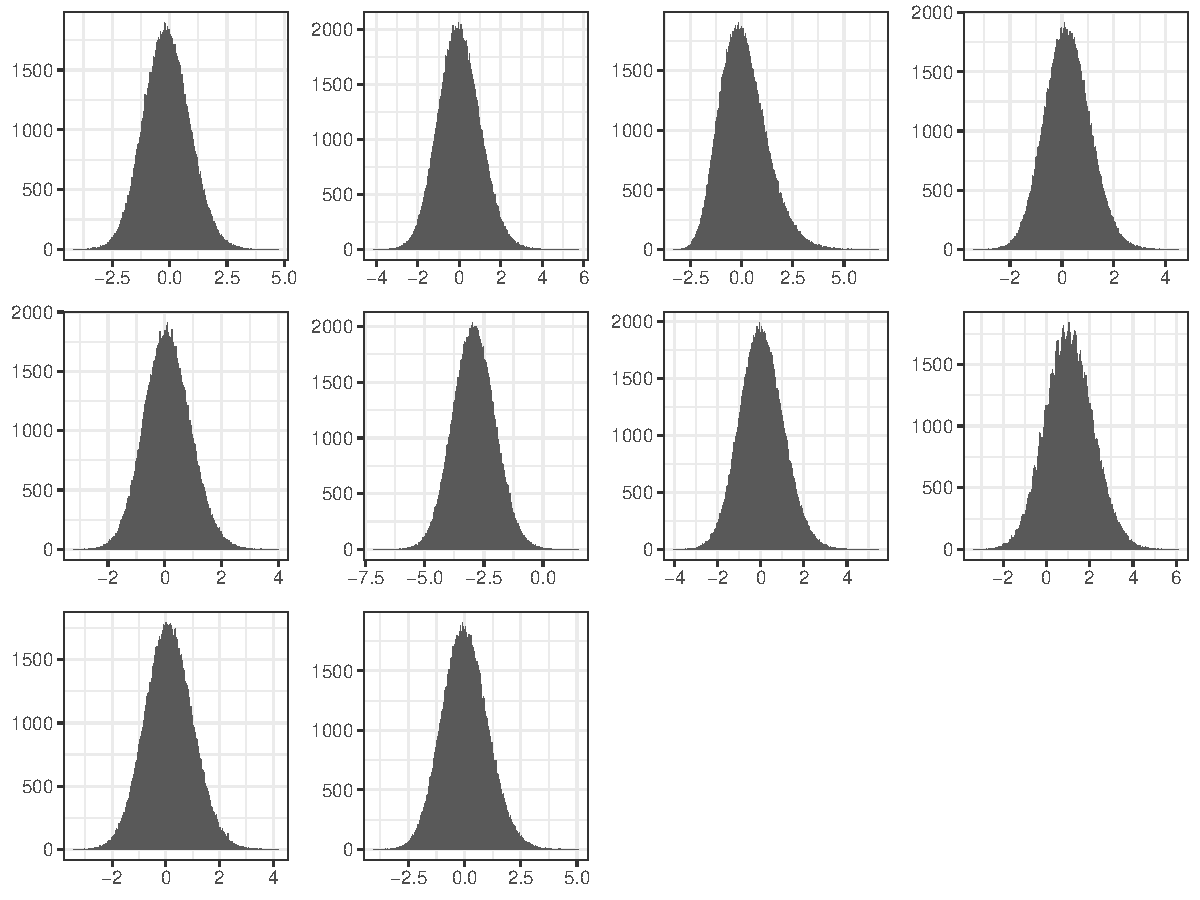
\includegraphics[width = \textwidth]{figures/papalexi_eccite_screen_gene_eff_ss_30.pdf}
	\caption{Papalexi data (effective sample size = 30).}
	\label{fig:papalexi-30}
\end{figure}

\clearpage

\section{Ideas for approximating the resampling distributions}

In an ideal world, we would be able to approximate all of the resampling distributions using sufficiently complex parametric models. However, my preliminary attempts to fit mixture models to these distributions failed, because the bumps get smaller as one goes further into the tails. These increasingly important bumps are modeled increasingly poorly, as they comprise decreasing proportions of the data. Therefore, especially in the short run, it seems clear that we should avoid modeling the bumpy parts of the resampling distributions. For distributions with some bumps, perhaps it is still possible to model their non-bumpy portions. The remaining questions then are (1) how to identify the non-bumpy portions of distributions, (2) how to model those portions, and (3) how to get $p$-values in the presence of bumpy-ness. 

Question 1 boils down to ``estimating'' the complement of the bumpy region $\mathcal B^c$ for a given resampling distribution. This is probably hard, but a heuristic is fix a quantile $\alpha_0 \in (0,1)$ (e.g. 0.01), and \textit{check} whether $[0, \alpha_0] \in \mathcal B^c$ and/or $[1-\alpha_0, 1] \in \mathcal B^c$. This might take the form of fitting some non-bumpy distribution to the corresponding tails and then test for goodness of fit. For Question 2, it is unclear whether is makes sense to differentiate between entirely non-bumpy distributions and partially non-bumpy distributions. For the former, we could attempt to model the entire distribution or just the tail(s), whereas for the latter we must model only the tail(s). Perhaps for the sake of a unified approach, we could model only the tail(s) of all distributions, avoiding the global modeling of resampling distributions entirely. As Tim suggests, the generalized Pareto distribution (GPD) is a good initial choice for modeling non-bumpy tails. For Question 3, the only apparent choice is to use empirical $p$-values. 

From the above discussion, the following outline of a strategy emerges. Draw $B_0$ samples. Compute initial empirical $p$-values $p^0_{\text{left}, \text{emp}}$ and $p^0_{\text{right}, \text{emp}}$, and define an initial two-tailed empirical $p$-value $p^0_{\text{emp}} \equiv 2\min(p^0_{\text{left}, \text{emp}}, p^0_{\text{right}, \text{emp}})$. If $p^0_{\text{emp}} > \alpha_0$ for some threshold $\alpha_0 \in (0,1)$, then stop and return $p^0_{\text{emp}}$. Otherwise, draw $B_1$ new samples. Based on the $B_1$ new samples, compute new empirical $p$-values $p^1_{\text{left}, \text{emp}}$ and $p^1_{\text{right}, \text{emp}}$. If $p^1_{\text{left}, \text{emp}} > 0.5$, define $p_{\text{left}} \equiv p^1_{\text{left}, \text{emp}}$. If $p^1_{\text{left}, \text{emp}} < 0.5$, then fit a GPD distribution to the quantiles of the data below some fixed $\alpha_1 \in (0,1)$. Test for goodness of fit. If the fit is good, define $p_{\text{left}}$ via this GPD distribution. Otherwise, define $p_{\text{left}} \equiv p^1_{\text{left}, \text{emp}}$. Carry out the same procedure to obtain $p_{\text{right}}$. Define $p \equiv 2 \cdot \min(p_{\text{left}}, p_{\text{right}})$. 

The tuning parameters of the above procedure are $B_0, B_1, \alpha_0, \alpha_1$. $B_0$ and $\alpha_0$ should be small enough that the procedure is fast, but large enough that small $p$-values make it beyond the first stage of the procedure. $B_1 \cdot \alpha_1$ (the number of samples used to fit the GPD) should be large enough that the GPD distribution fit is good and there is enough power to detect bumpy alternatives in the goodness of fit test. On the other hand, $B_1$ should be small enough that computation is fast, and $\alpha_1$ should be small enough that $[0,\alpha_1]$ (or $[1-\alpha_1, 1]$) is contained in $\mathcal B^c$ if the left (or right) tail is non-bumpy. I estimate that we'll need something in the ballpark of $(B_0, B_1, \alpha_0, \alpha_1) \equiv (5000, 50000, 0.1, 0.1)$. If resamples are cheap, we can do away with the first stage entirely, and always draw some large-ish number of resamples like 50,000. If fitting the GPD distribution is expensive, then we can fit it only when the empirical $p$-values for the large sample are small enough. 

\end{document}
